%---------------- Main window ---------------------
\section{Main Window}

Niget's graphical user interface (GUI) can be started by running the \texttt{niget} (\texttt{niget.exe}) executable. Using two optional parameters \emph{filename} and \emph{fileformat} (currently available options: \emph{niget}, \emph{unht}, \emph{hysitron}), a file of a given type is opened on application start by running \texttt{niget -f fileformat filename}.

The main window shows all currently available methods as different tabs and a row of general function buttons. The tabs are inactive at the start of the program and get activated when a file is opened.

\begin{figure}[ht]
  \centering
  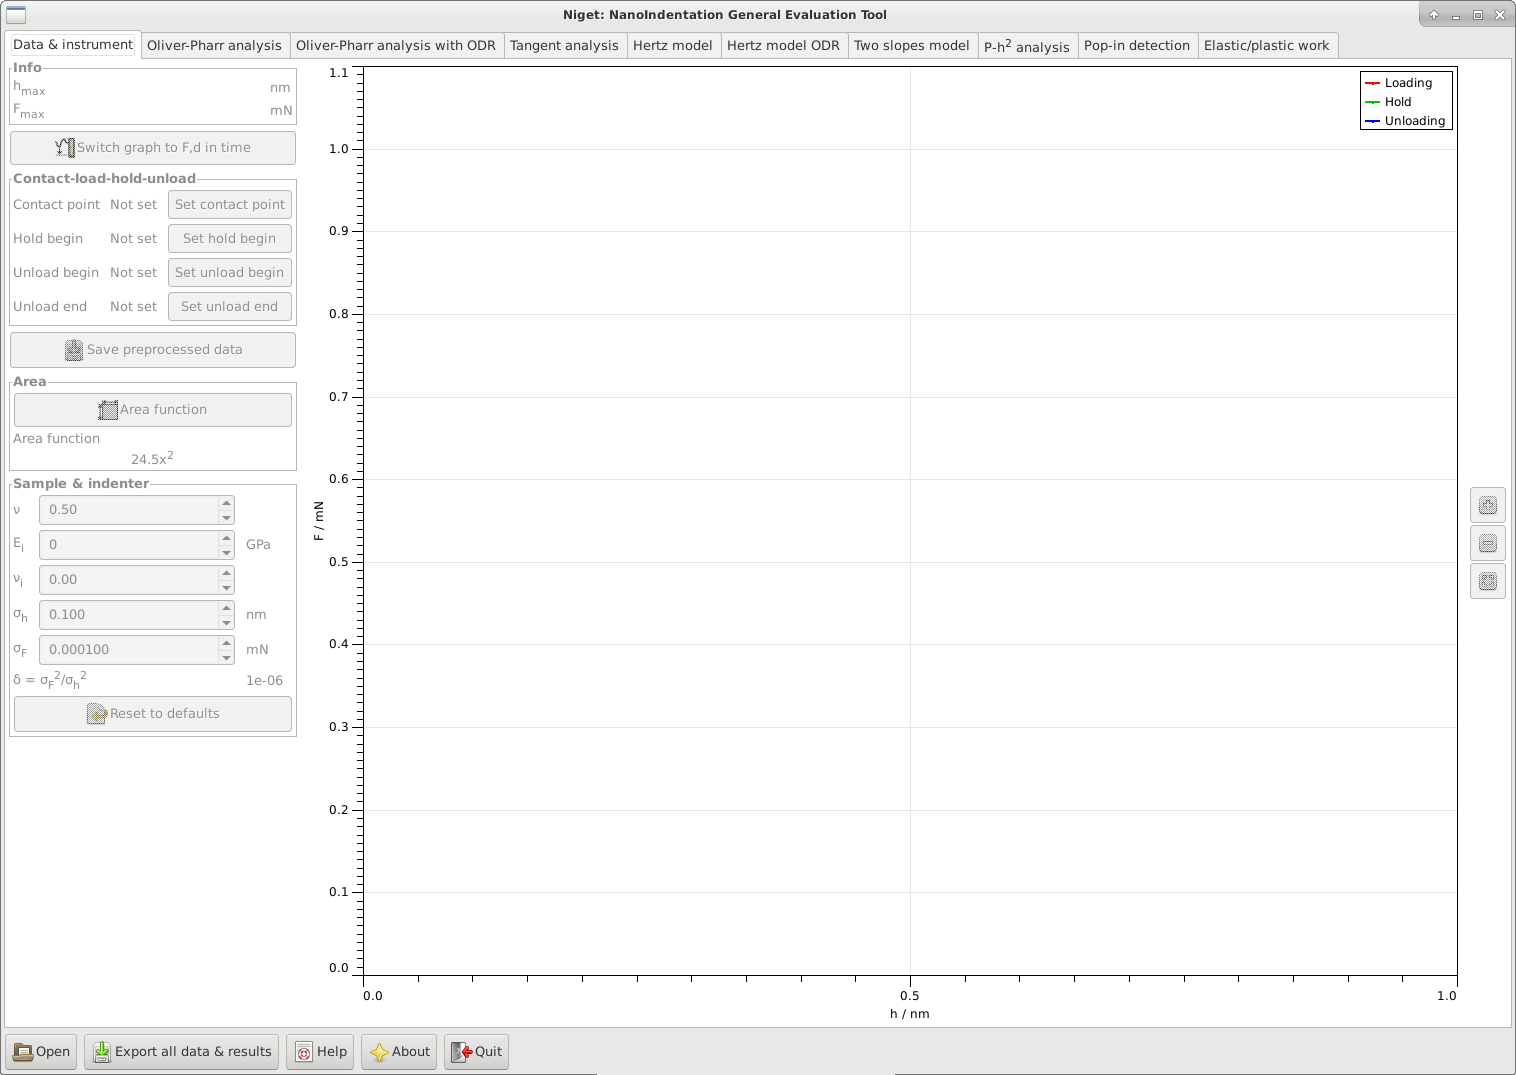
\includegraphics[width=\textwidth]{images/screen-main}
  \caption{Main window}
\end{figure}

The buttons are:
\begin{itemize}
 \item \emph{Open:} Load a file in a chosen format. Currently, only files of one of the predefined plain-text formats. can be opened. 
 Each file should contain only one loading-unloading curve. Files with more than one indentation should load as well, but the behaviour may be ``surprising''. Currently, only the decimal point is supported as the decimal mark.
 Lines that do not correspond to the given format, because they are, e.g., empty or hold comments, are skipped. \\
 WARNING: The units MUST agree with the given format or you will get nonsense numerical results! 
 
 \begin{itemize}
 \item[-] \verb|Time (s)  Depth (nm)  Load (mN)|: first three columns correspond to time (which is skipped), depth in nm and load in mN.
 \item[-] \verb|Time (s)  Depth (nm)  Load (uN)|: first three columns correspond to time (which is skipped), depth in nm and load in $\mu$N.
 \item[-] \verb|Depth (nm)  Load (uN)|: first two columns correspond to depth in nm and load in $\mu$N.
 \item[-] \verb|Depth (nm)  Load (mN)|: first two columns correspond to depth in nm and load in mN.
 \item[-] \verb|Load (mN)  Depth (nm)|: first two columns correspond to load in mN and depth in nm.
 \item[-] \verb|Load (uN)  Depth (nm)|: first two columns correspond to load in $\mu$N and depth in nm.
 \item[-] \verb|Niget|: native format of Niget.
 \end{itemize}
 The file cannot be loaded if it's not in the given format or if it contains \verb|inf| or \verb|nan| values. The data are supposed to be sufficiently comprehensive in order to define the contact point as well the loading and unloading part.

 \item \emph{Export all data \& results:} Save the processed indentation data and  results from all methods. The user chooses a basename to which a suffix is appended for each method. A file is created even if there are no meaningful results for a method. 
                    %Results of uncertainty analysis and Monte Carlo calculations are saved as well.
 \item \emph{Help:} Open HTML documentation in an associated browser.
 \item \emph{About:} Display additional information about the software.
 \item \emph{Quit:} Exit the program.
\end{itemize}

Note that when the program exits (either by pressing \emph{Quit} or closing the main window), no results are saved. \\
The program keeps its own few settings for user comfort. These are saved in \verb|niget_settings.cfg| in the user configuration directory. 
